\chapter{Experimental Procedure and Results of Polymerase Modeling} % (fold)
\label{cha:experimental_results_of_polymerase_modeling}
The procedure for performing an experiment with the model for polymerase directionality evolution consists of constructing an environment for the model to operate on, then setting the model running for a set number of time steps. Various parameters of the simulation are reported at set intervals during the run. Because a number of the dynamical systems in the model depend on randomly generated numbers, each experiment was carried out in 10 copies to smooth fluctuations, and all of the values reported represent a numerical average of all 10 runs. All plots were generated using the R software package\cite{Ihaka:1996p1018}.

The dynamics included in the model for polymerase directionality should generate scale free results. That is, the evolution of traits should show the same dynamics regardless of population size or genome length. In this model, the only trait capable of evolving is polymerase rate, so in order to verify that the dynamics were indeed scale free, the first experiments carried out were designed to investigate simple dynamics of polymerase rate evolution over a range of scales. One experiment consisted of starting populations of 10 organisms and a maximum population (environmental carrying capacity) of 1000 organisms combined with 4 different genome lengths as described in table~\ref{tab:scale_length}.

\begin{table}
	\begin{center}
		\begin{tabular}[c]{ l | l | l | l }
			Temp. ($t$) & Starting Pop. & Max Pop. & Genome Length \\
			\hline
			0.40 & 10 & 1000 & 10 \\
			0.40 & 10 & 1000 & 100 \\
			0.40 & 10 & 1000 & 1000 \\
			0.40 & 10 & 1000 & 10000 \\
		\end{tabular}
		\caption{Determining genome length scale effects.}
		\label{tab:scale_length}
	\end{center}
\end{table}

In order to avoid a founder bias with regards to polymerase rate, in each experiment the ten organisms in each seed population consisted of one organism of each of the ten possible polymerase rates. The simulation temperature of 0.40 was chosen because it results in a significant amount of error, and therefore variability due to mutations, during growth but is not a high enough temperature that certain other temperature effects begin to alter growth and evolution. The results from this experiment are plotted in figure~\ref{fig:scale_length}.

\begin{figure}[h]
	\centering
		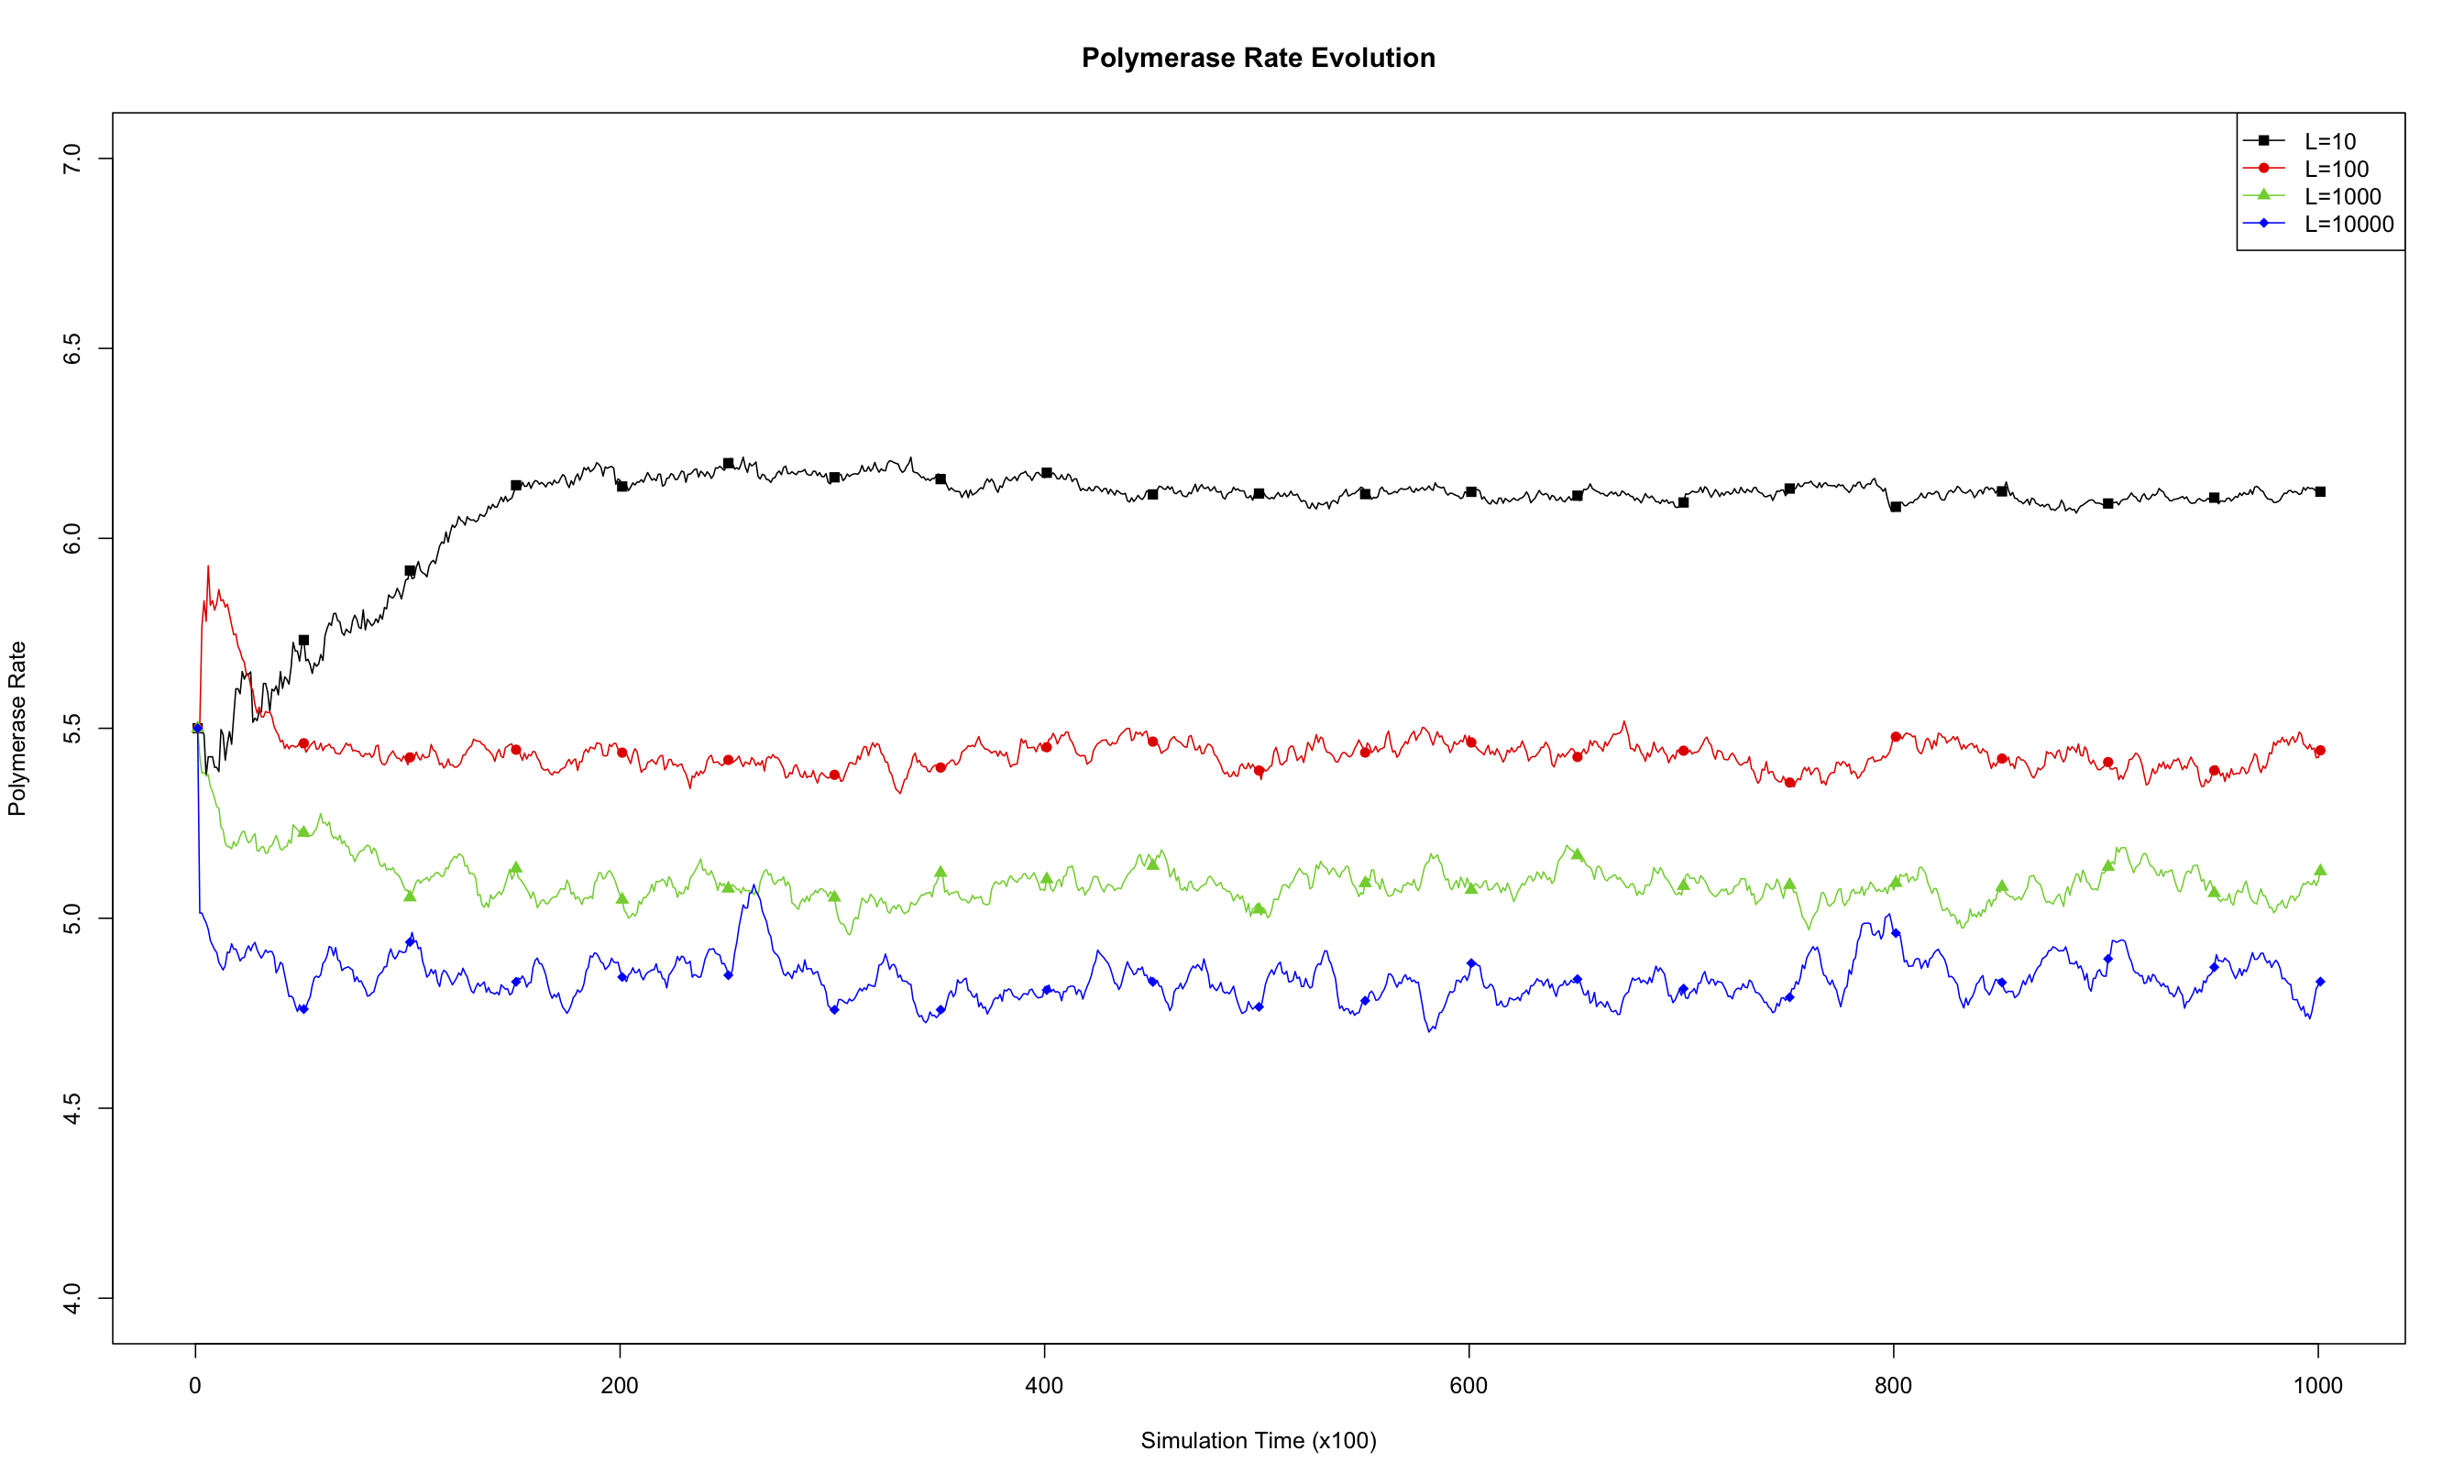
\includegraphics[width=\textwidth]{scale_length}
	\caption{\textbf{Effects of Genome Length on Polymerase Rate Evolution.} The average polymerase rate for the entire simulation population is plotted against simulation time steps (each unit on the abscissa is equivalent to 100 simulation time steps). The organisms each had genomes of length 10, 100, 1000, or 10000.}
	\label{fig:scale_length}
\end{figure}

Second, a set of experiments were carried out to investigate the effect of population size on the evolution of polymerase rate. In this experiment, the genome length of the organisms in each environment was held constant at 1000, the starting population was set to 10, and the maximum population was set to either 100, 1000, 10000, or 100000. As in the first set of experiments, the starting population in each environment was seeded with organisms with polymerase rates evenly distributed in the range 1-10 and the simulation temperature was set to 0.40. Table~\ref{tab:scale_num} summarizes these experiments.

\begin{table}
	\begin{center}
		\begin{tabular}[c]{ l | l | l | l }
			Temp. ($t$) & Starting Pop. & Max Pop. & Genome Length \\
			\hline
			0.40 & 10 & 100 & 1000 \\
			0.40 & 10 & 1000 & 1000 \\
			0.40 & 10 & 10000 & 1000 \\
			0.40 & 10 & 100000 & 1000 \\
		\end{tabular}
		\caption{Determining size scale effects.}
		\label{tab:scale_num}
	\end{center}
\end{table}

Figure~\ref{fig:scale_num} is a plot of the average polymerase rate of the population in each environment against the simulation time. Based on these initial experiments, it was decided that a maximum population size of 1000 with a genome length of 1000 could serve as an adequate representative of the dynamics over the range of possible values. These values were chosen because they also keep the size of the simulations reasonable with regards to the amount of computational time required to run each simulation, since the run time of the simulations scale with the population size and organisms with longer genomes require more time-steps to achieve the same number of doublings as organisms with shorter genomes.

\begin{figure}[h]
	\centering
		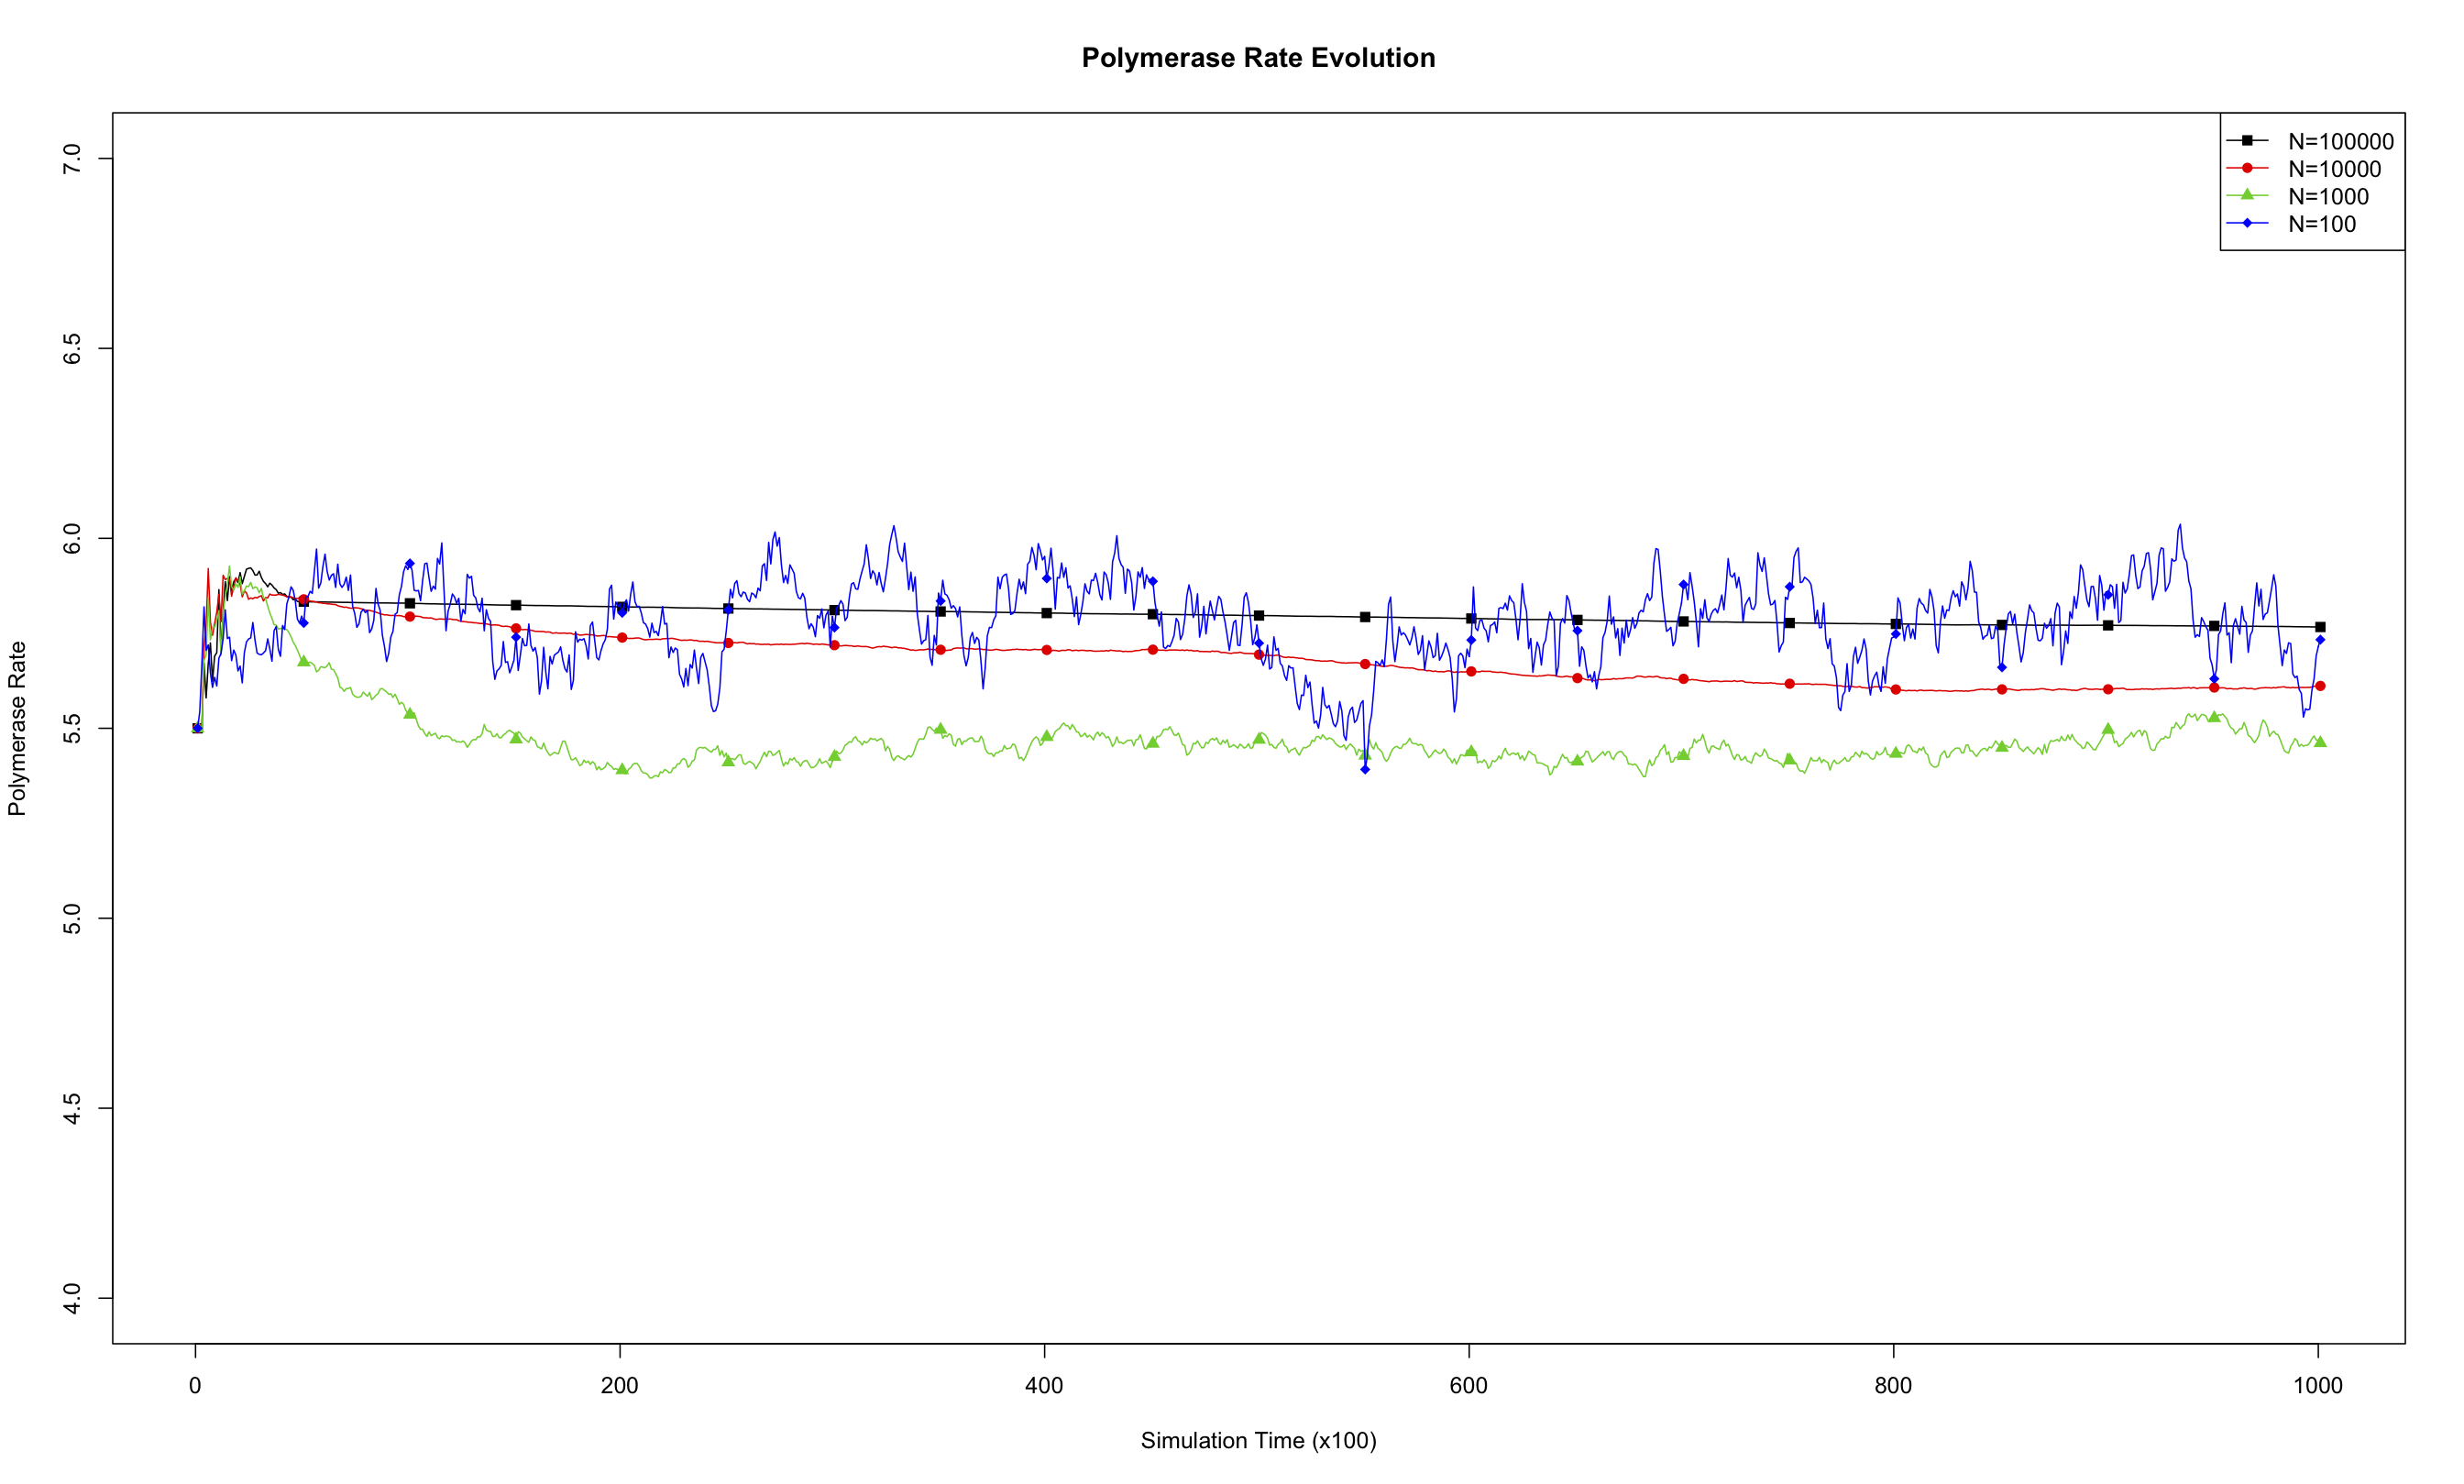
\includegraphics[width=\textwidth]{scale_num}
	\caption{\textbf{Effects of Environmental Carrying Capacity on Polymerase Rate Evolution.} The average polymerase rate for the entire simulation population is plotted against simulation time steps (each unit on the abscissa is equivalent to 100 simulation time steps). The organisms each had a genome length of 1000, and the environments had a maximum capacity ($N$) of 100, 1000, 10000, or 100000 organisms.}
	\label{fig:scale_num}
\end{figure}

Finally, in order to validate the model and how reasonably it simulates the observed growth dynamics of biological organisms, a set of experiments were carried out starting with small populations of 10 organisms, as before, and following their growth at different temperatures. The first two sets of experiments described above were only carried out with forward polymerizing organisms. To be sure that model organisms with reverse, $3'\to5'$, polymerases had growth dynamics similar to forward polymerizing organisms, these experiments were carried out using both types of organisms. Table~\ref{tab:temp_incr} summarizes the parameters used for these experiments.

\begin{table}
	\begin{center}
		\begin{tabular}[c]{ l | l | l | l }
			Temp. ($t$) & Max Pop. & Genome Length & Directionality \\
			\hline
			0.10 & & &\\
			0.30 & & & forward \\
			0.40 & 1000 & 1000 &\\
			0.60 & & &\\
			\hline
			0.10 & & &\\
			0.30 & & & reverse \\
			0.40 & 1000 & 1000 &\\
			0.60 & & &\\
		\end{tabular}
		\caption{Growth dynamics at various temperatures.}
		\label{tab:temp_incr}
	\end{center}
\end{table}

The results of these simulations are presented in figure~\ref{fig:temp_incr_mut}. Simulations were carried out for each type of polymerase individually so that only the dynamics of the polymerase would influence growth. The simulations were also run disallowing mutations. Under this condition there can be no change in polymerase rate for an individual and its daughters from one generation to the next. These results are presented in figure~\ref{fig:temp_incr_nomut}. We monitored both the population rate and the average polymerase rate for all the organisms in the environment.

\begin{figure}[!ht]
	\begin{center}
		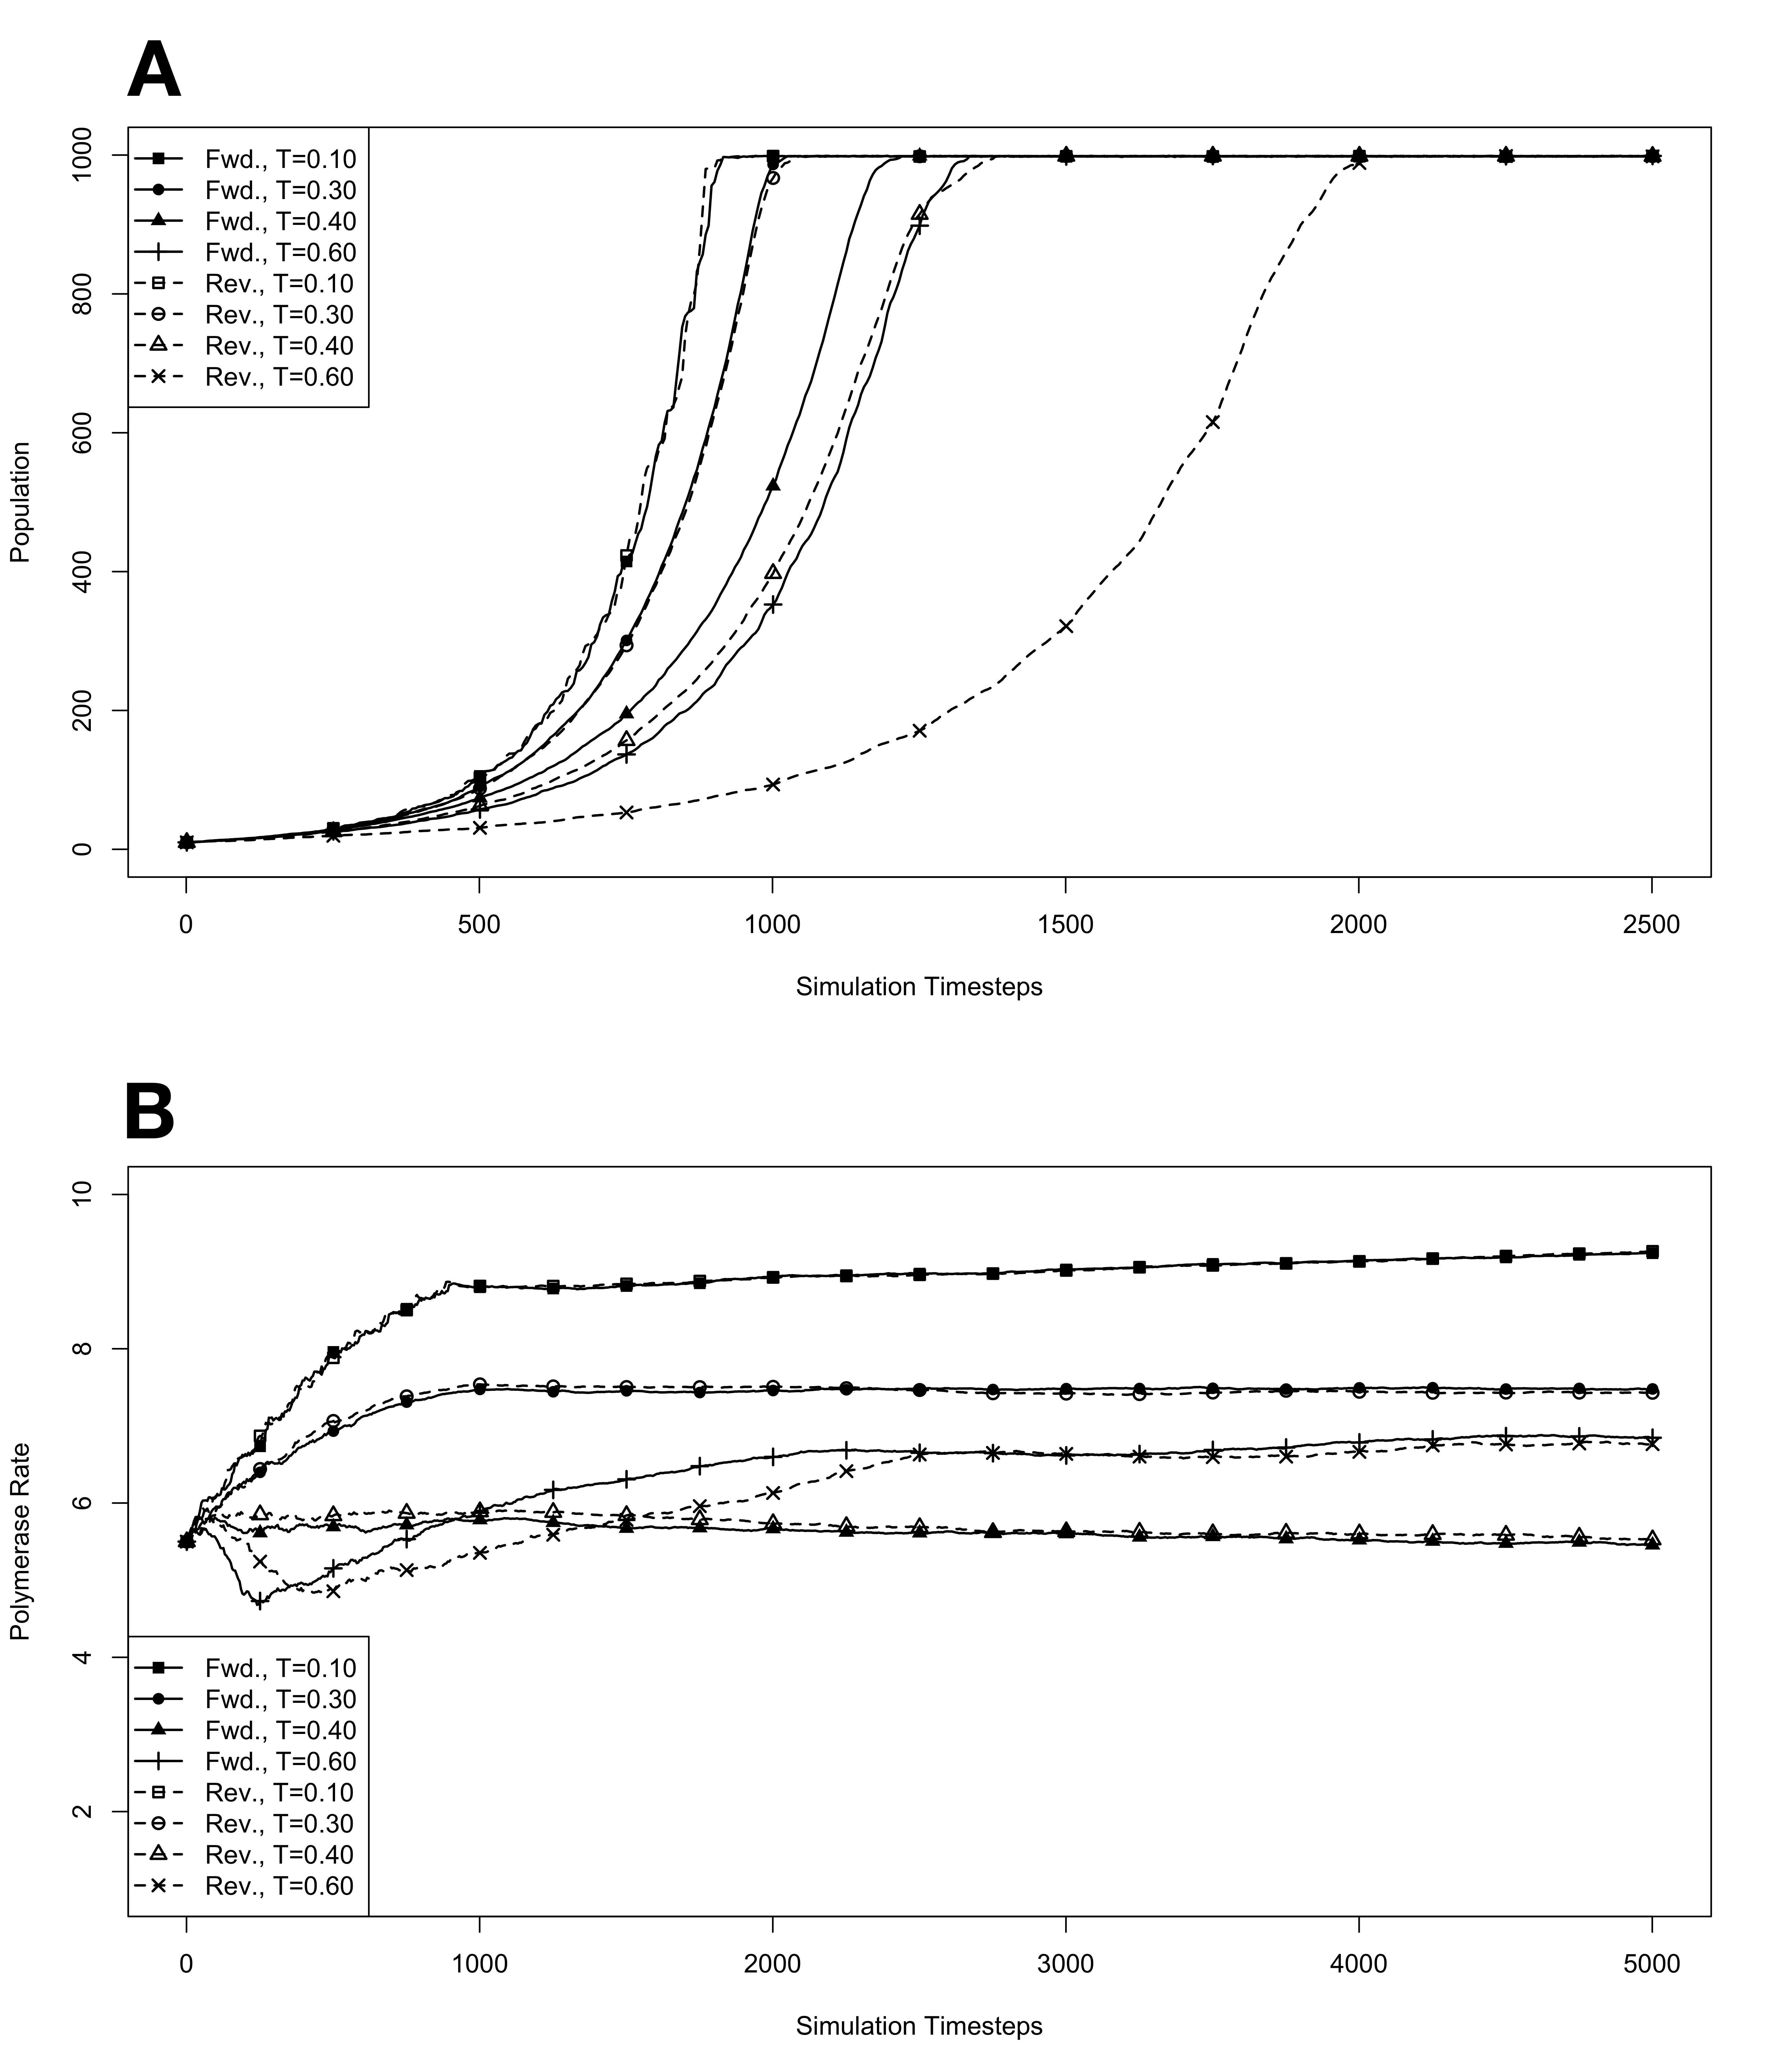
\includegraphics[width=0.95\textwidth]{temp_incr_mut}
	\end{center}
	\caption{
	{\bf Exponential growth at various temperatures in the absence of competition, with mutations.}  The model system was seeded with environments, at simulation temperatures of 0.10, 0.30, 0.40, or 0.60, containing 10 organisms with a 5.5 average polymerase rate. \textbf{A}. Population size of model organisms as a function of simulation time. \textbf{B}. Evolution of the average polymerase rate for the organisms in each environment as a function of simulation time. In each case, solid lines are used to indicate environments with forward polymerizing organisms and dashed lines are for reverse polymerizing organisms. Different temperatures are indicated with different data markers as indicated in the figure legend, and are expressed in units of $\frac{\Delta E}{R}$.
	}
	\label{fig:temp_incr_mut}
\end{figure}

\begin{figure}[!ht]
	\begin{center}
		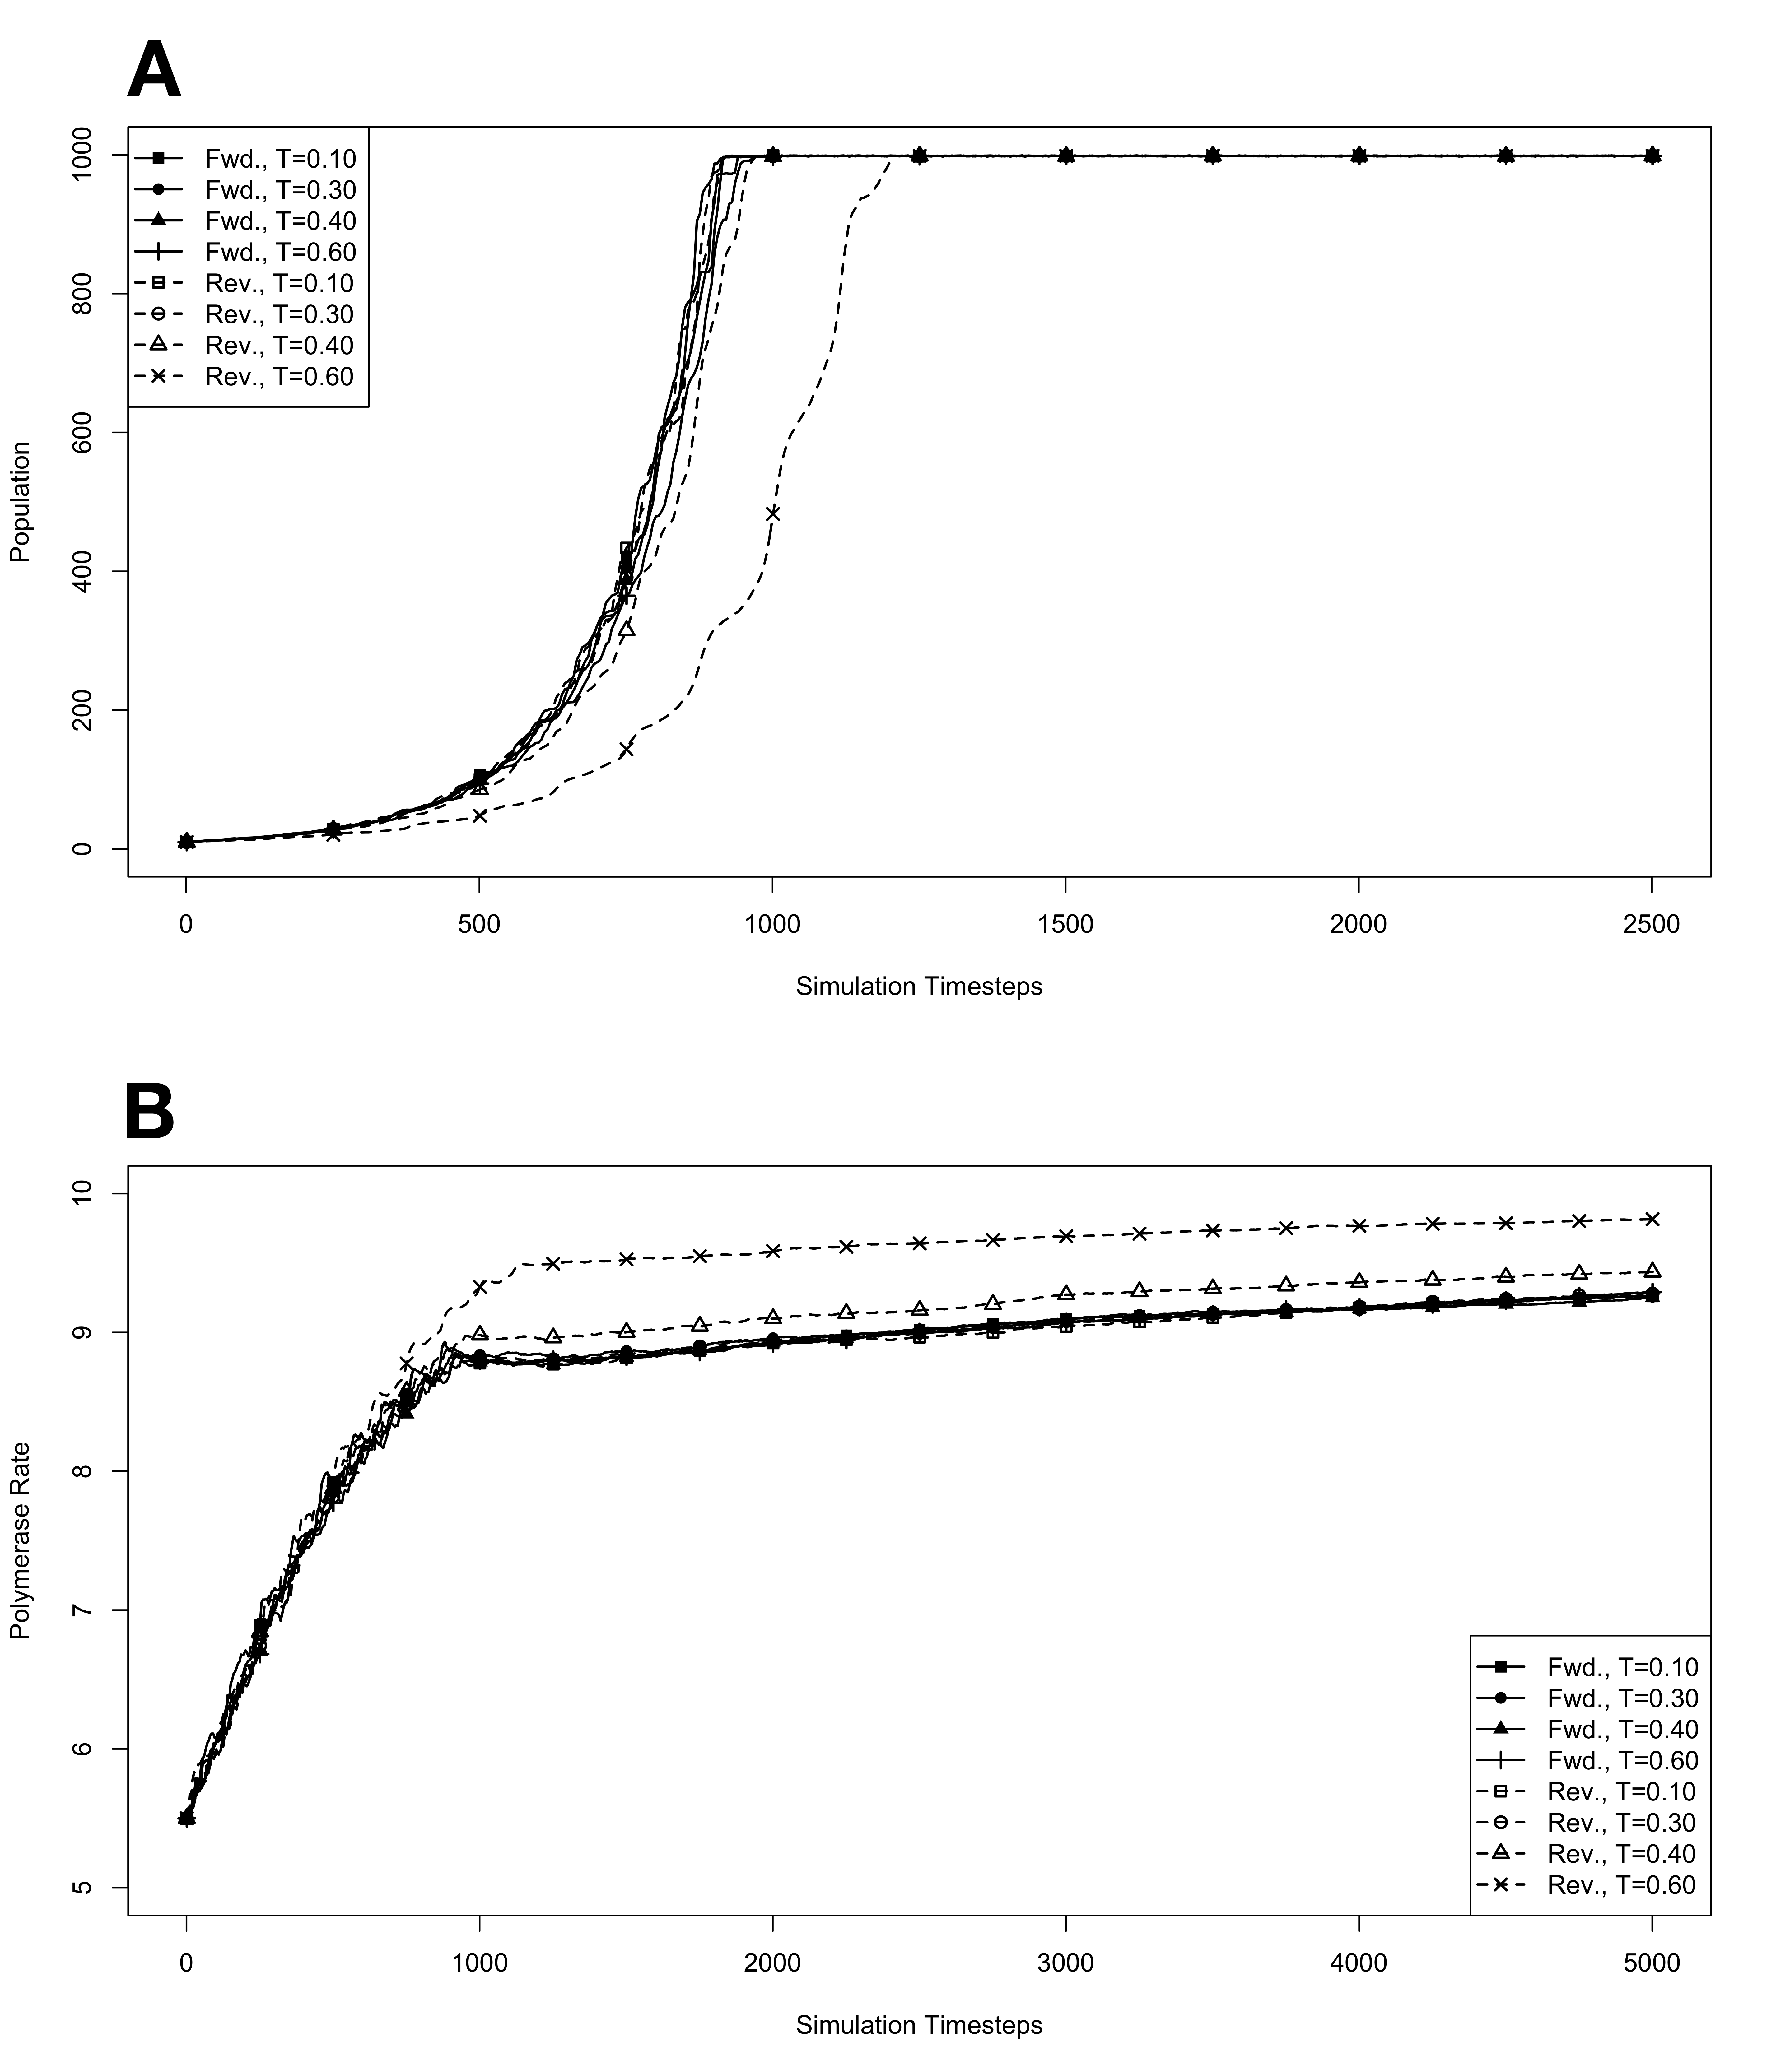
\includegraphics[width=0.95\textwidth]{temp_incr_nomut}
	\end{center}
	\caption{
	{\bf Exponential growth at various temperatures in the absence of competition, with no mutations.}  The model system was seeded with environments, at simulation temperatures of 0.10, 0.30, 0.40, or 0.60, containing 10 organisms with a 5.5 average polymerase rate. \textbf{A}. Population size of model organisms as a function of simulation time. \textbf{B}. Evolution of the average polymerase rate for the organisms in each environment as a function of simulation time. In each case, solid lines are used to indicate environments with forward polymerizing organisms and dashed lines are for reverse polymerizing organisms. For every simulation mutations were disallowed. Different temperatures are indicated with different data markers as indicated in the figure legend, and are expressed in units of $\frac{\Delta E}{R}$.
	}
	\label{fig:temp_incr_nomut}
\end{figure}


\subsubsection*{Evolution During Exponential Growth}
In each of the experiments performed up to this point, forward or reverse organisms were allowed to grow in isolation. In order to gain some insight into the dynamics of polymerase evolution, it is necessary to set these two classes of model organisms in competition with each other. When considering the competition of organisms, there are two domains which are interesting to probe. The first is the competition of the organisms as they explore a new ecological niche. That is, the way in which organisms compete during phases of exponential growth. The second is the competition that occurs when an environment is already at its carrying capacity. It would be expected that an evolutionary strategy which results in the most rapid growth should dominate during exponential growth. It is also conceivable that such a strategy might not represent the most efficient use of resources available and therefore might ultimately loose out to a different strategy when growth is limited by resources.

We investigated how organisms with forward or reverse polymerases would behave when competing with each other for resources during an exponential growth phase. To do this, we seeded environments with 100 organisms, where 50 of the organisms contained forward polymerases and 50 reverse. For each type, there were 5 organisms with each possible polymerase rates for an average starting polymerase rate of 5.5. Table~\ref{tab:growth_compet} summarizes the parameters used for these experiments.

\begin{table}
	\begin{center}
		\begin{tabular}[c]{ l | l | l | c }
			Temp. ($t$) & Max Pop. & Genome Length & Seed organisms \\
			\hline
			0.10 & & & 50 forward\\
			0.30 & & & and\\
			0.40 & 1000 & 1000 & 50 reverse\\
			0.60 & & &\\
		\end{tabular}
		\caption{Competitive growth at various temperatures.}
		\label{tab:growth_compet}
	\end{center}
\end{table}

The results of these simulations are presented in figure~\ref{fig:growth_compet_mut}. Simulations were again replicated disallowing mutations. These results are presented in figure~\ref{fig:growth_compet_nomut}. In each environment, we tracked the subpopulations of organisms with forward and reverse polymerases separately so that we could follow the population changes and polymerase rate evolution for each condition in the mixed case independently.

\begin{figure}[!ht]
	\begin{center}
		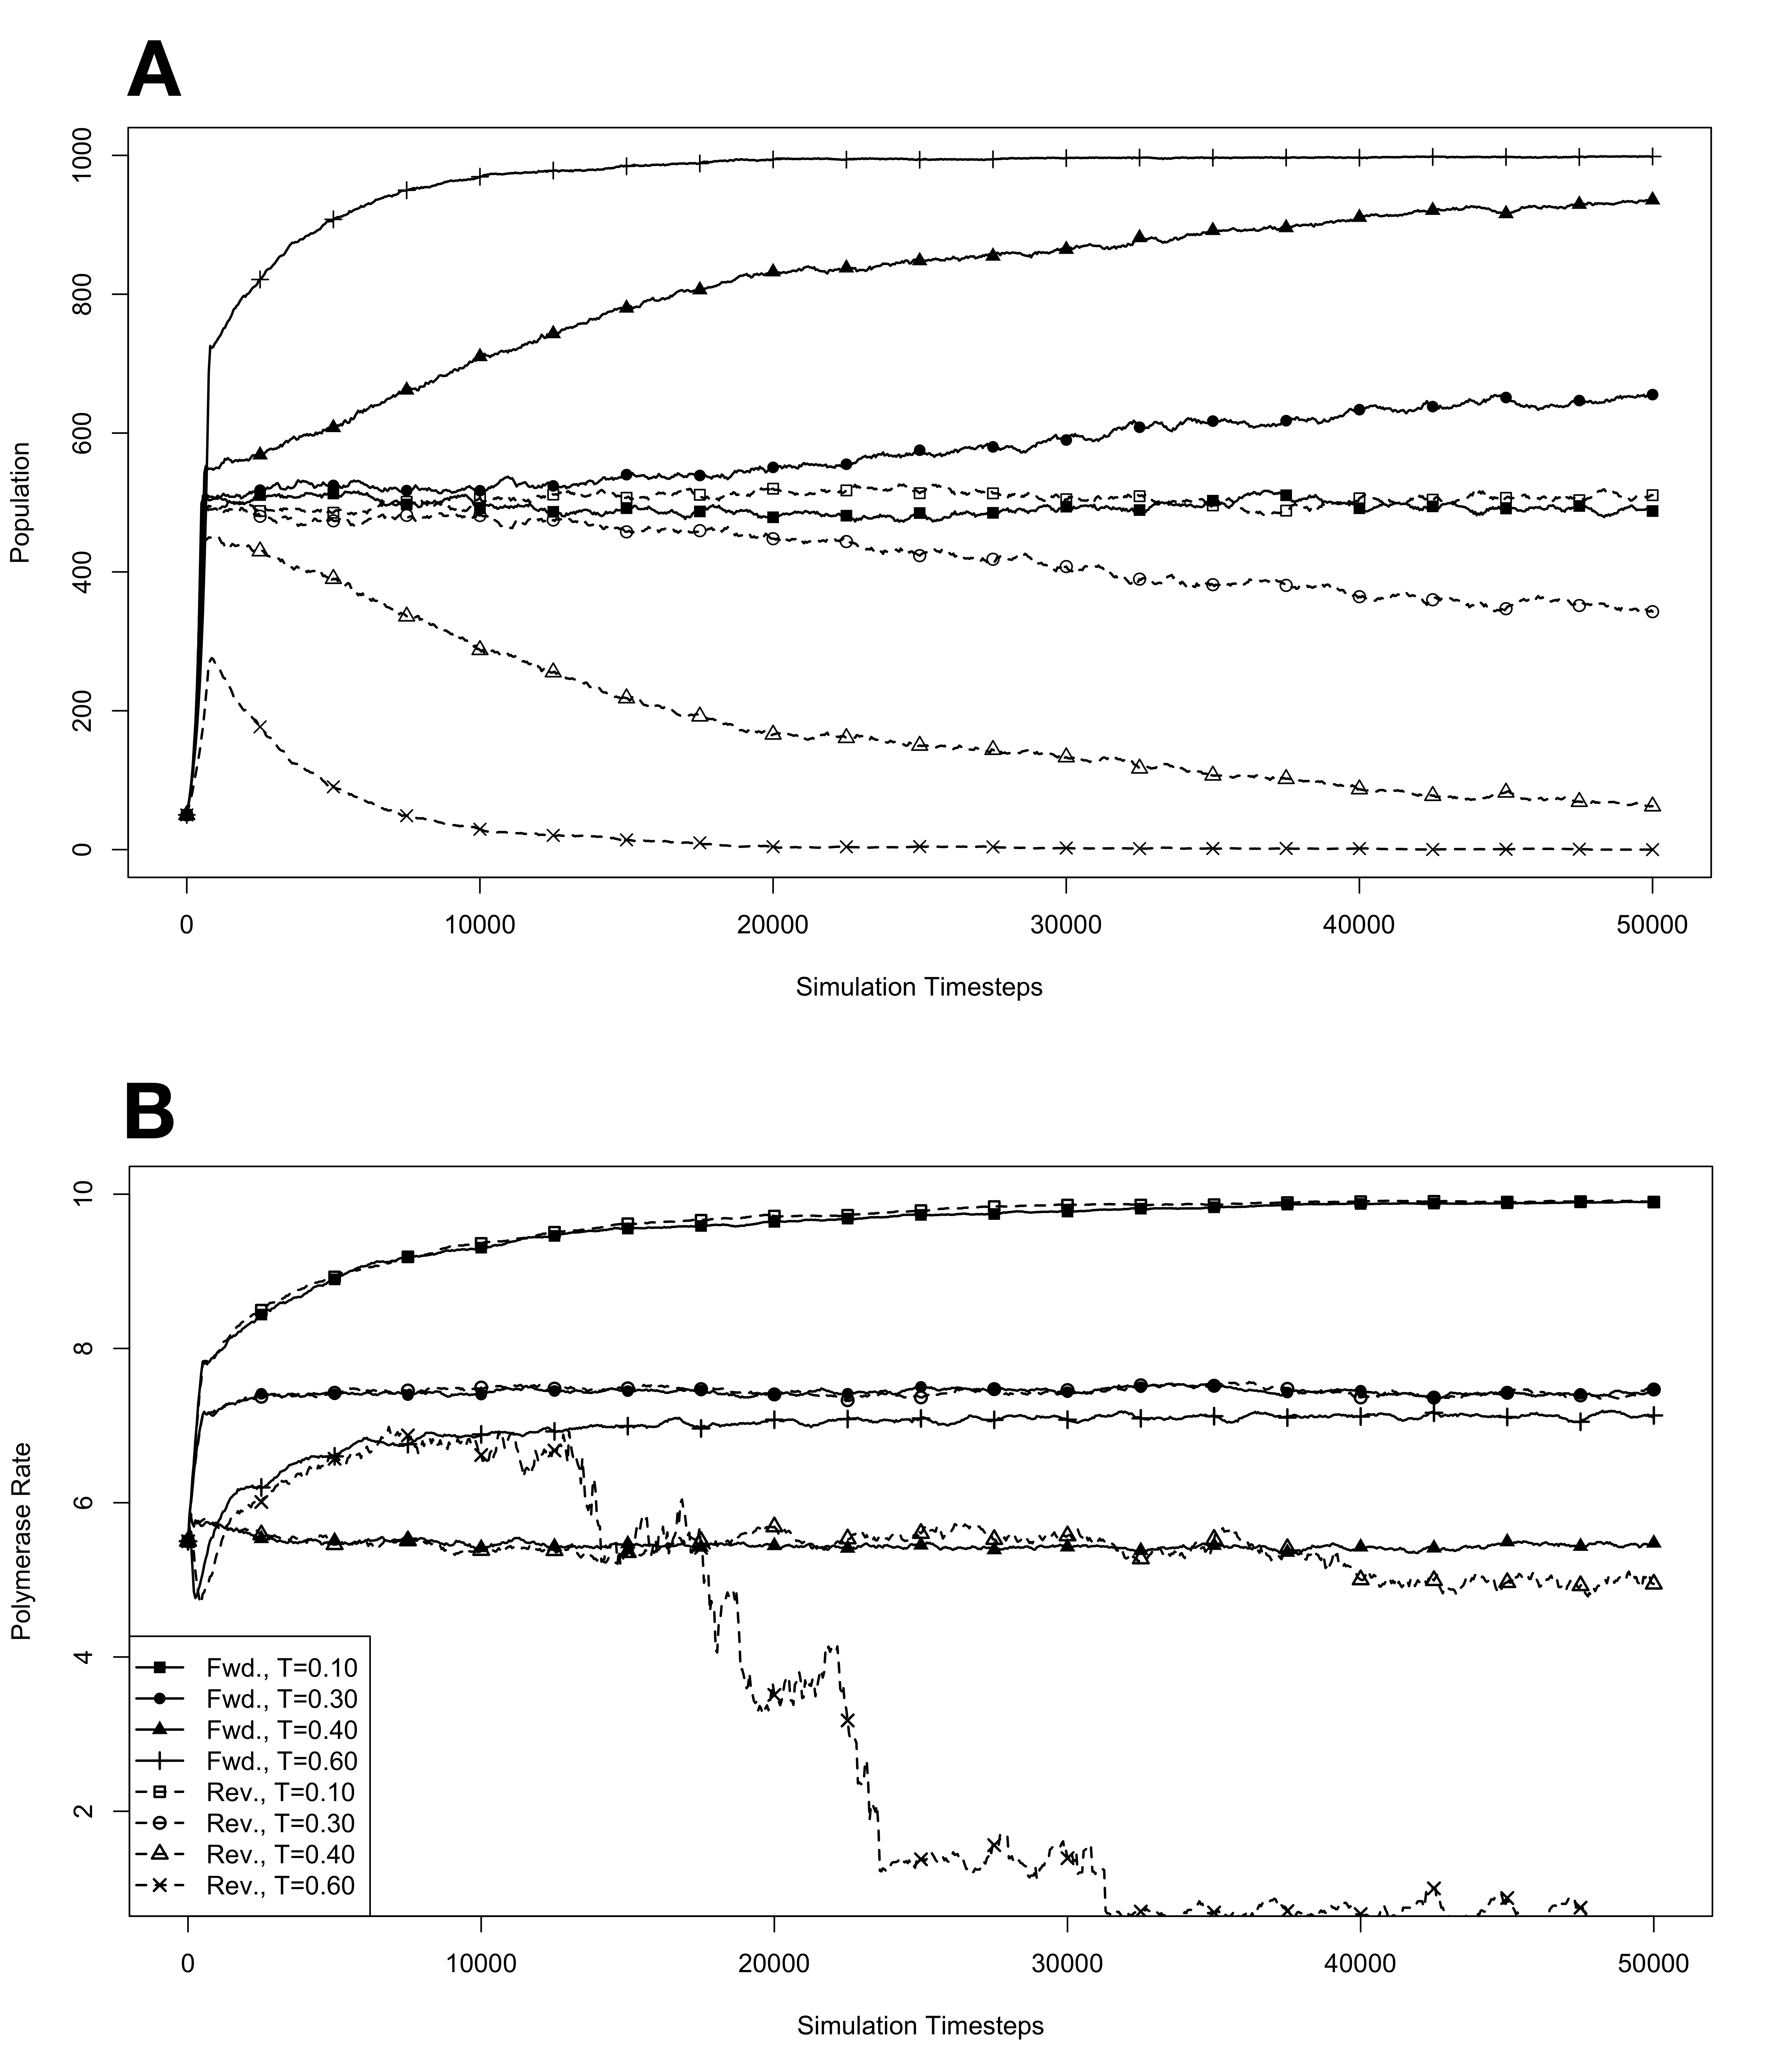
\includegraphics[width=0.95\textwidth]{growth_compet_mut}
	\end{center}
	\caption{
		{\bf Competition during exponential growth at various temperatures, with mutations.}  The model system was seeded with environments, at simulation temperatures of 0.10, 0.30, 0.40, or 0.60, containing 100 organisms, 50 each with forward and reverse polymerases, with a 5.5 average polymerase rate. \textbf{A}. Population size of model organisms as a function of simulation time. \textbf{B}. Evolution of the average polymerase rate for the organisms in each environment as a function of simulation time. In each case, solid lines are used to indicate environments with forward polymerizing organisms and dashed lines are for reverse polymerizing organisms. Different temperatures are indicated with different data markers as indicated in the figure legend, and are expressed in units of $\frac{\Delta E}{R}$.
		}
		\label{fig:growth_compet_mut}
\end{figure}

\begin{figure}[!ht]
	\begin{center}
		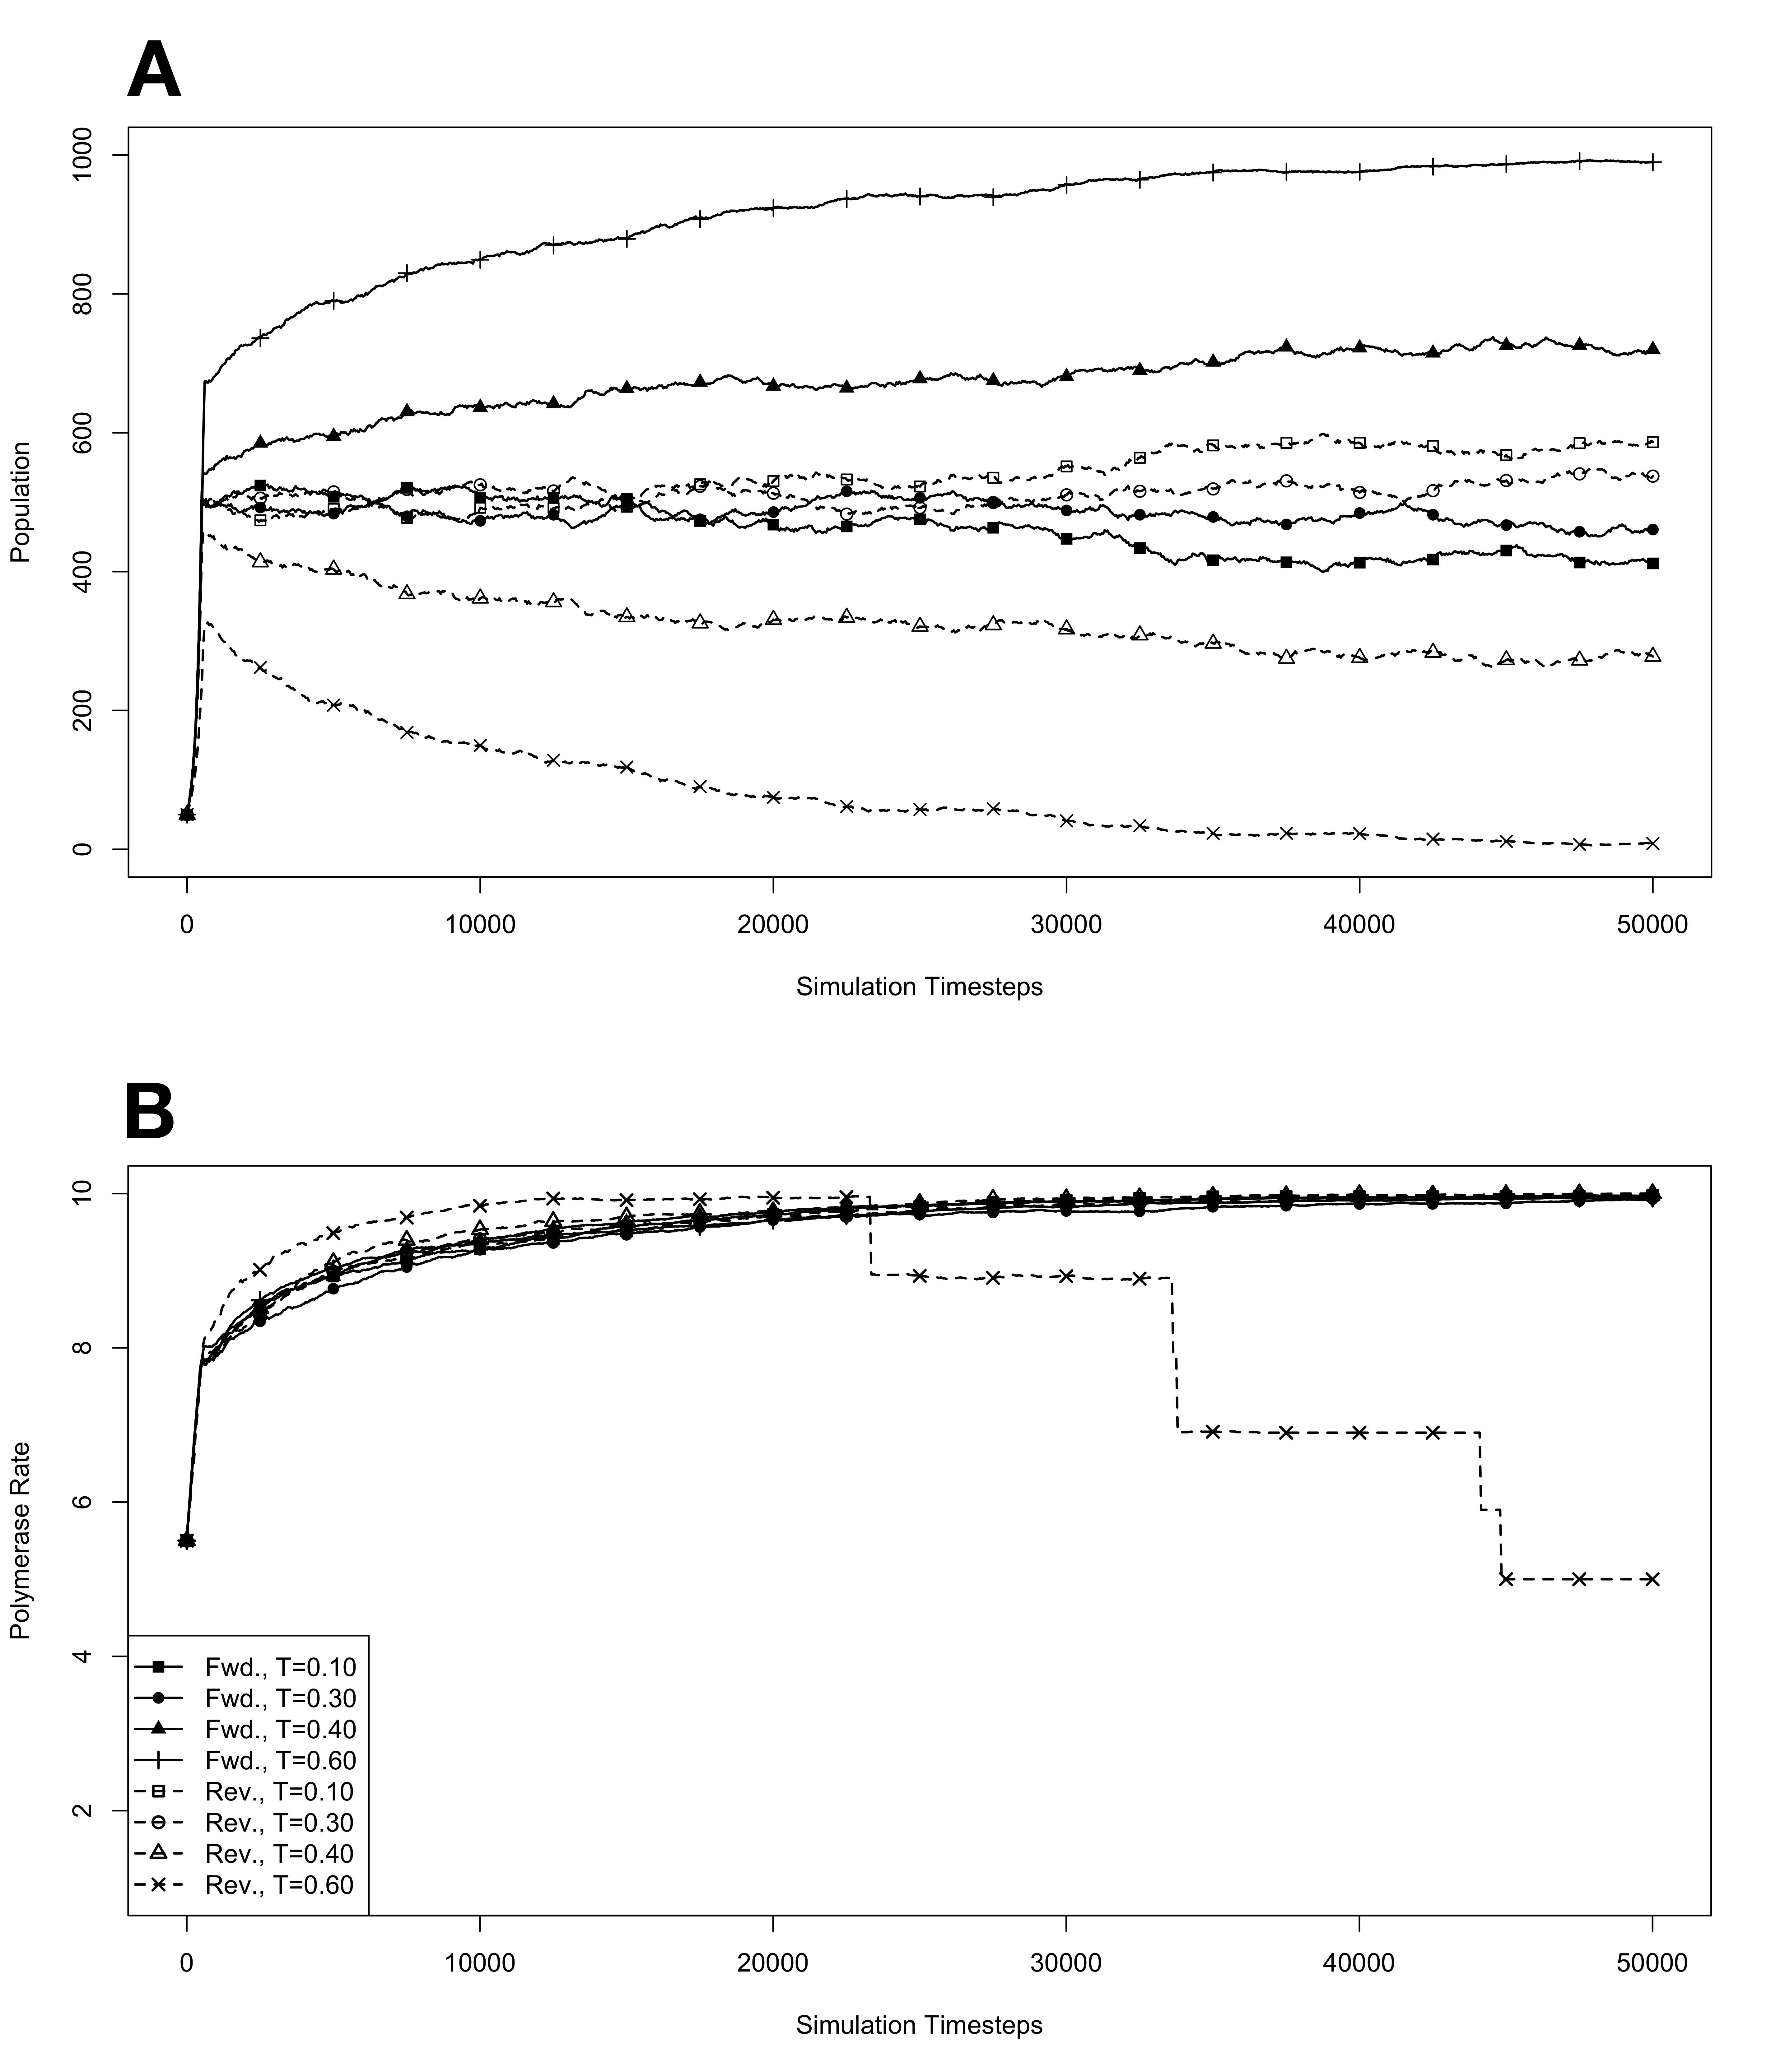
\includegraphics[width=0.95\textwidth]{growth_compet_nomut}
	\end{center}
	\caption{
		{\bf Competition during exponential growth at various temperatures, with no mutations.}  The model system was seeded with environments, at simulation temperatures of 0.10, 0.30, 0.40, or 0.60, containing 100 organisms, 50 each with forward and reverse polymerases, with a 5.5 average polymerase rate. \textbf{A}. Population size of model organisms as a function of simulation time. \textbf{B}. Evolution of the average polymerase rate for the organisms in each environment as a function of simulation time. In each case, solid lines are used to indicate environments with forward polymerizing organisms and dashed lines are for reverse polymerizing organisms. For every simulation mutations were disallowed. Different temperatures are indicated with different data markers as indicated in the figure legend, and are expressed in units of $\frac{\Delta E}{R}$.
		}
		\label{fig:growth_compet_nomut}
\end{figure}

\subsubsection*{Competition in a Full Environment}
To further investigate how organisms with forward polymerases fared in competition with organisms with reverse polymerases, specifically to see if an equilibrium was possible between the two varieties, we performed a number of simulations starting with an environment already at its maximum capacity. This was done by seeding each environment with 500 organisms containing forward polymerases and 500 containing reverse. For each variety, there were 50 organisms seeded with each of the 10 possible polymerase rates. Table~\ref{tab:strict} summarizes the parameters used for these experiments.

\begin{table}
	\begin{center}
		\begin{tabular}[c]{ l | l | l | c }
			Temp. ($t$) & Max Pop. & Genome Length & Seed organisms \\
			\hline
			0.10 & & & 500 forward\\
			0.30 & & & and\\
			0.40 & 1000 & 1000 & 500 reverse\\
			0.60 & & &\\
		\end{tabular}
		\caption{Competitive growth in a full environment at various temperatures.}
		\label{tab:strict}
	\end{center}
\end{table}

The results of these simulations are presented in figure~\ref{fig:strict_compet_mut}. As before, these conditions were repeated with mutations disallowed, and those results are presented in figure~\ref{fig:strict_compet_nomut}.

\begin{figure}[!ht]
	\begin{center}
		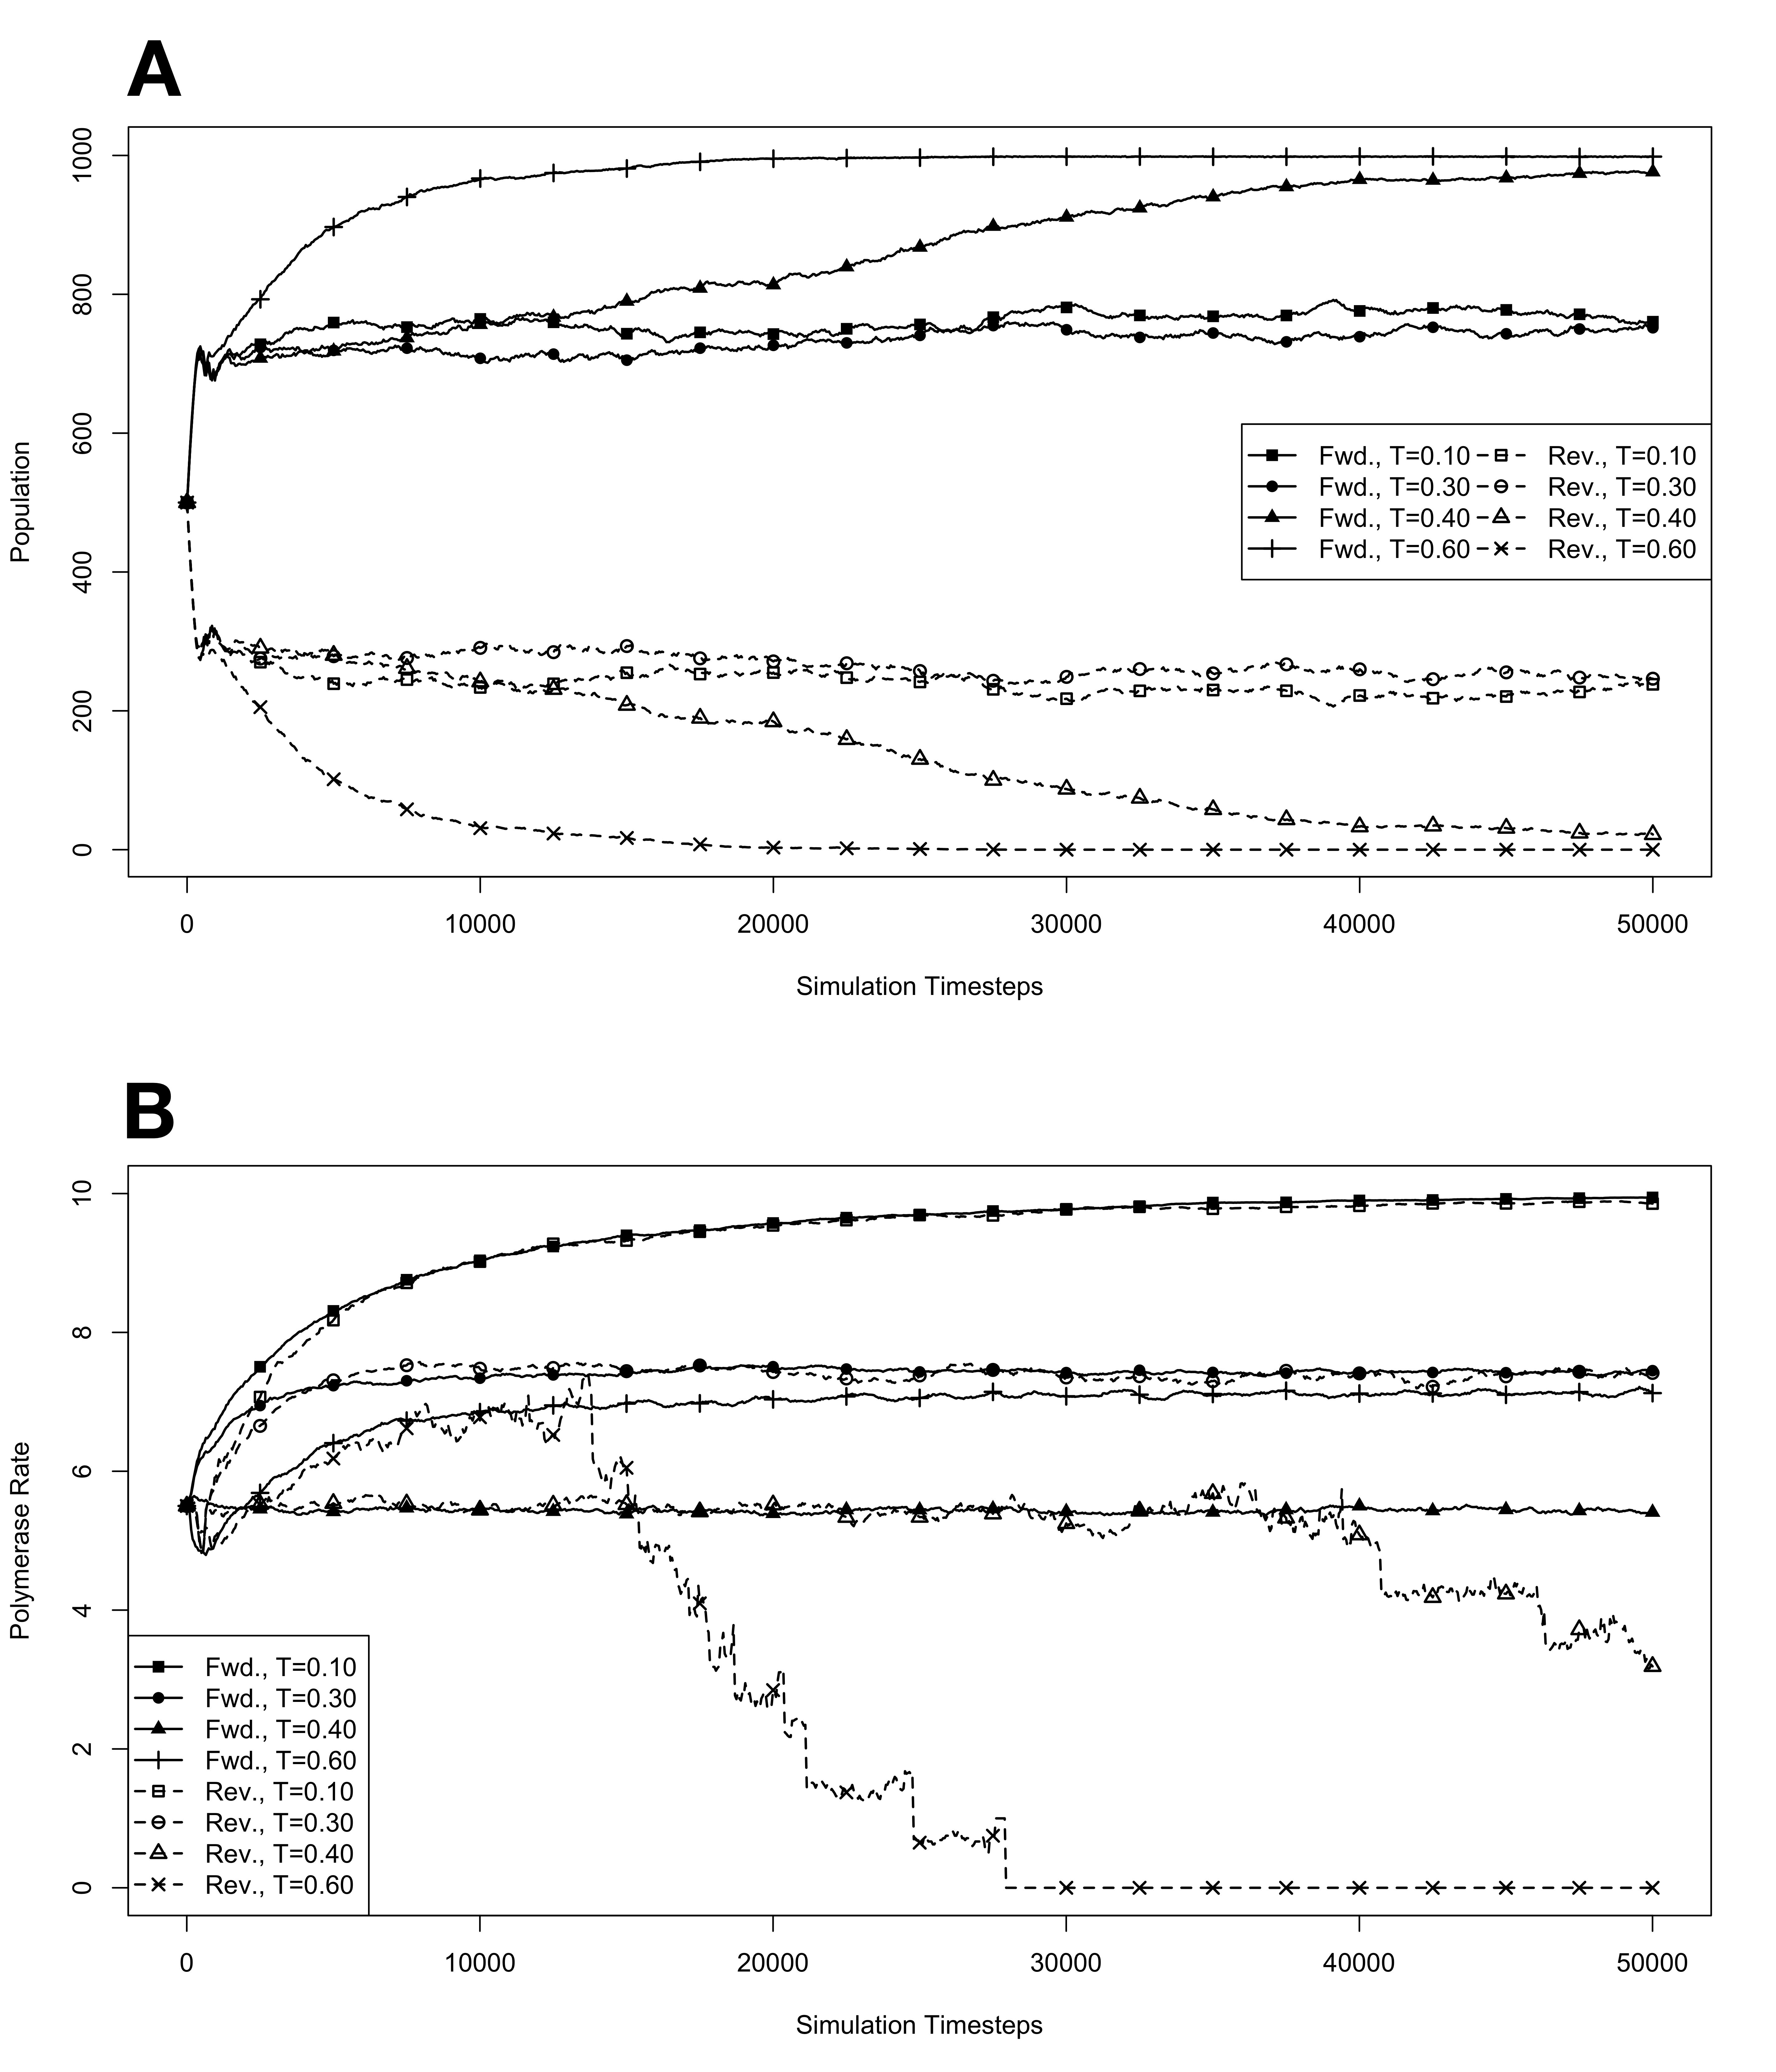
\includegraphics[width=0.95\textwidth]{strict_compet_mut}
	\end{center}
	\caption{
		{\bf Competition in an environment at maximum capacity, with mutations.}  Environments, at simulation temperatures of 0.10, 0.30, 0.40, or 0.60, were seeded with 500 organisms containing forward polymerases and 500 containing reverse, both with a 5.5 average polymerase rate. \textbf{A}. Population size of model organisms as a function of simulation time. \textbf{B}. Evolution of the average polymerase rate for the organisms in each environment as a function of simulation time. In each case, solid lines are used to indicate environments with forward polymerizing organisms and dashed lines are for reverse polymerizing organisms. Different temperatures are indicated with different data markers as indicated in the figure legend, and are expressed in units of $\frac{\Delta E}{R}$.
		}
		\label{fig:strict_compet_mut}
\end{figure}

\begin{figure}[!ht]
	\begin{center}
		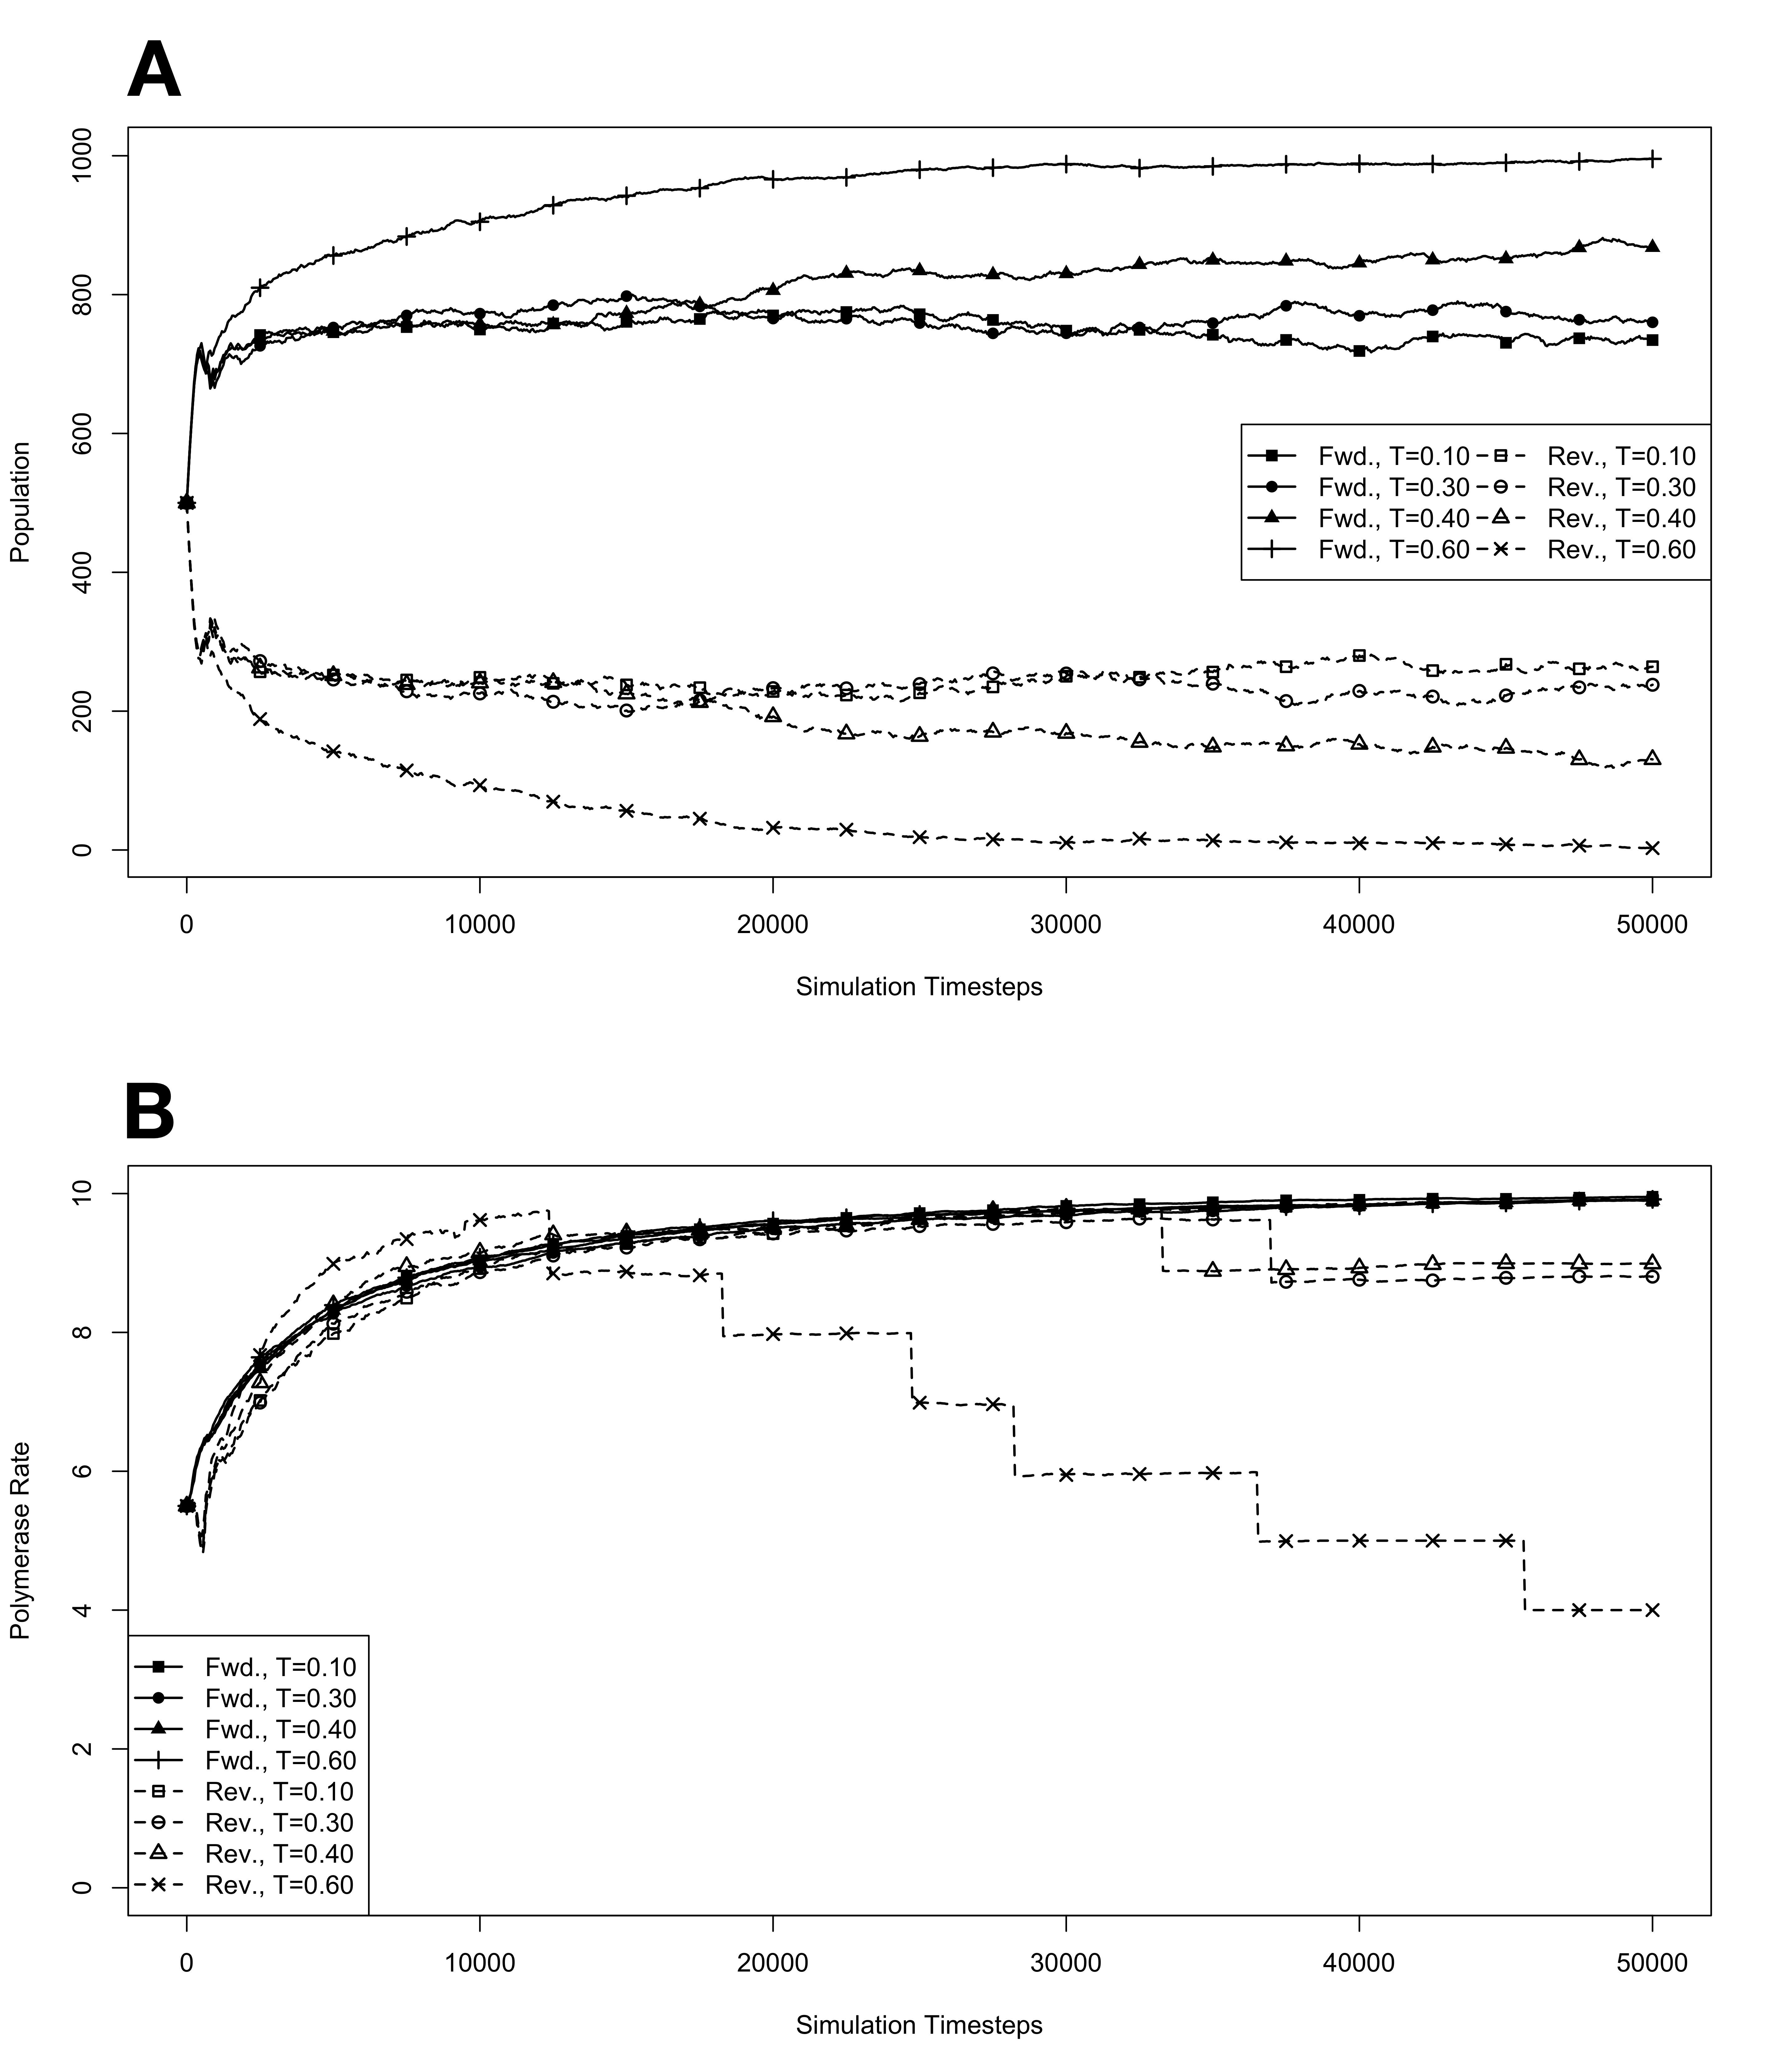
\includegraphics[width=0.95\textwidth]{strict_compet_nomut}
	\end{center}
	\caption{
		{\bf Competition in an environment at maximum capacity, with no mutations.}  Environments, at simulation temperatures of 0.10, 0.30, 0.40, or 0.60, were seeded with 500 organisms containing forward polymerases and 500 containing reverse, both with a 5.5 average polymerase rate. \textbf{A}. Population size of model organisms as a function of simulation time. \textbf{B}. Evolution of the average polymerase rate for the organisms in each environment as a function of simulation time. In each case, solid lines are used to indicate environments with forward polymerizing organisms and dashed lines are for reverse polymerizing organisms. For every simulation mutations were disallowed. Different temperatures are indicated with different data markers as indicated in the figure legend, and are expressed in units of $\frac{\Delta E}{R}$.
		}
		\label{fig:strict_compet_nomut}
\end{figure}

We noted that the results of this last experiment seemed to indicate that, when mutations were allowed, their might be a temperature regime in which there is a transition between an equilibrium of organisms containing forward and reverse polymerases and a complete dominance by organisms containing the forward polymerase. To get a more detailed picture of this transition temperature, we repeated the simulations with full environments at temperatures from 0.10 to 0.60 in 0.05 increments. Table~\ref{tab:strict_log} summarizes the parameters used for these experiments, and figure~\ref{fig:strict_compet_log} shows the results of these simulations.

\begin{table}
	\begin{center}
		\begin{tabular}[c]{ l | l | l | c }
			Temp. ($t$) & Max Pop. & Genome Length & Seed organisms \\
			\hline
			0.10 & & &\\
			0.15 & & &\\
			0.20 & & & 500 forward\\
			0.25 & & &\\
			0.30 & & &\\
			0.35 & 1000 & 1000 & and\\
			0.40 & & &\\
			0.45 & & &\\
			0.50 & & & 500 reverse\\
			0.55 & & &\\
			0.60 & & &\\
		\end{tabular}
		\caption{Competitive growth in a full environment at many finely divided temperatures.}
		\label{tab:strict_log}
	\end{center}
\end{table}

\begin{figure}[!ht]
	\begin{center}
		\includegraphics[width=0.95\textwidth]{strict_compet_log}
	\end{center}
	\caption{
		{\bf Competition in an environment at maximum capacity at various temperatures.}  Simulations were carried out with environments at temperatures ranging from 0.10 to 0.60 in 0.05 increments. In each simulation, the environment was seeded at full capacity with 500 organisms containing forward polymerases and 500 containing reverse. For each variety there were 50 organisms with each of the possible polymerase rates, giving an average rate of 5.5 In \textbf{A} and \textbf{B} the natural log of the population of organisms containing reverse polymerases is plotted as a function of simulation time. \textbf{A} is the data from simulations where mutation was allowed, and \textbf{B} is from simulations where mutations were not permitted. A plot of the slopes of a least squares regression line for the data in each simulations is plotted as a function of simulation temperature. Data from simulations with mutation is plotted as the solid line with data from the no mutation simulations plotted as a dashed line.
		}
		\label{fig:strict_compet_log}
\end{figure}
% chapter experimental_results_of_polymerase_modeling (end)